\setcounter{section}{0}
\section{Lý thuyết}
\subsection{Động lượng của một vật}
\begin{minipage}{0.6\textwidth}
	Động lượng $\vec{p}$ của một vật khối lượng $m$ đang chuyển động với vận tốc $\vec{v}$ là đại lượng được xác định bởi công thức:
	\begin{equation*}
		\vec{p}=m\vec{v}.
	\end{equation*}
	Động lượng là một đại lượng vector cùng hướng với vận tốc của vật.
\end{minipage}
\begin{minipage}{0.4\textwidth}
	\begin{center}
		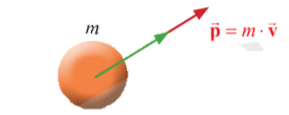
\includegraphics[scale=0.7]{../figs/G10-023-1}
	\end{center}
\end{minipage}

\ppgiai{
	\begin{description}
		\item[Bước 1] Ta xác định vector vận tốc của vật dựa vào kiến thức đã học về chuyển động 
		
		+ Độ lớn của vận tốc.
		
		+ Phương chiều của vận tốc.
		\item[Bước 2]Biết được vector vận tốc của vật ta tính được động lượng của vật
		
		+ Độ lớn của động lượng là tích khối lượng và độ lớn vận tốc (kg $\cdot$ m/s).
		
		+ hướng của động lượng chính là hướng của vận tốc.
	\end{description}
}
\subsection{Tổng động lượng của hệ vật}
%\vspace{-0.5cm}
\subsubsection{Động lượng hệ nhiều vật}

Động lượng của hệ là tổng động lượng của các vật trong hệ

\begin{equation*}
	\vec {p} = \vec {p_1} + \vec{p_2}+\vec{p_3}+...
\end{equation*}

\subsubsection{Hệ cô lập (hay hệ kín)}

Một hệ nhiều vật được gọi là hệ cô lập (hay hệ kín) khi không có ngoại lực tác dụng lên hệ hoặc nếu có thì các ngoại lực ấy cân bằng nhau.

\ppgiai{
	\begin{description}
		\item[Bước 1] Tìm vectơ động lượng của mỗi vật theo định nghĩa 
		\begin{equation*}
			\vec{p} = m \vec{v}.
		\end{equation*}
		Động lượng của hệ là một đại lượng vectơ có đặc điểm: 
		\begin{itemize}
			\item Phương và chiều: cùng phương cùng chiều với vận tốc của vật.
			\item Độ lớn: $p=mv$.
		\end{itemize} 
		\item [Bước 2] Vectơ động lượng hệ vật bằng tổng vectơ động lượng của các vật trong hệ:
		\begin{equation*}
			\vec {p} = \vec {p_1} + \vec{p_2}+\vec{p_3}+...
		\end{equation*}
	\end{description}
}
\subsubsection{Các trường hợp đặc biệt}
\begin{itemize}
	\item \textbf{Trường hợp 1: Hai vectơ động lương cùng phương cùng chiều} 
	\begin{center}
		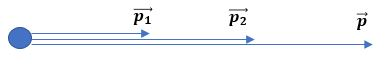
\includegraphics[scale=0.6]{../figs/VN10-PH-29-L-021-2-1.JPG}
	\end{center}
	\begin{equation*}
		\vec {p} = \vec {p_1} + \vec{p_2}.
	\end{equation*}
	
	Vectơ động lượng của hệ $\vec{p}$ có 
	\begin{itemize}
		\item Phương và chiều: cùng phương cùng chiều với vector động lượng của mỗi vật.
		\item Độ lớn: $$p=p_1+p_2.$$ 
	\end{itemize}
	
	\item \textbf{Trường hợp 2: Hai vectơ động lượng cùng phương ngược chiều}
	\begin{center}
		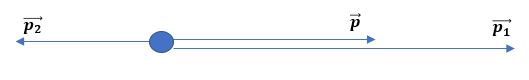
\includegraphics[scale=0.6]{../figs/VN10-PH-29-L-021-2-2.JPG}
	\end{center}
	\begin{equation*}
		\vec {p} = \vec {p_1} + \vec{p_2}.
	\end{equation*}
	Vectơ động lượng của hệ $\vec{p}$ có 
	\begin{itemize}
		\item Phương và chiều: cùng phương cùng chiều với vector động lượng của vật có giá trị lớn hơn.
		\item Độ lớn: $$p=|p_1-p_2|.$$
	\end{itemize}
	
	\item \textbf{Trường hợp 3: Hai vectơ động lượng vuông góc}
	\begin{center}
		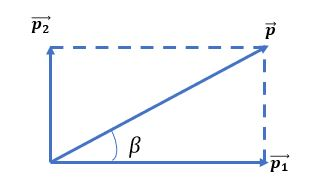
\includegraphics[scale=0.6]{../figs/VN10-PH-29-L-021-2-3.JPG}
	\end{center}
	\begin{equation*}
		\vec {p} = \vec {p_1} + \vec{p_2}.
	\end{equation*}
	Vectơ động lượng của hệ $\vec{p}$ có 
	\begin{itemize}
		\item Phương và chiều: là đường chéo của hình chữ nhật xác định bởi góc $\beta$ với $\tan \beta = {p_2}/{p_1}.$
		\item Độ lớn: $$p = \sqrt {p_1^2+p^2_2}.$$
	\end{itemize}
	Khi đó vector động lượng của hệ $\vec{p}$ có
	
	
	\item \textbf{Trường hợp 4: Hai vectơ động lượng tạo với nhau một góc $\alpha$}
	\begin{center}
		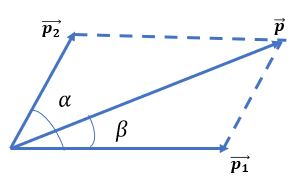
\includegraphics[scale=0.6]{../figs/VN10-PH-29-L-021-2-4.JPG}
	\end{center}
	\begin{equation*}
		\vec {p} = \vec {p_1} + \vec{p_2}.
	\end{equation*}
	Vectơ động lượng của hệ $\vec{p}$ có 
	\begin{itemize}
		\item Phương và chiều: là đường chéo của hình bình hành xác định bởi góc $\beta$ tính bởi 
		\begin{equation*}
			\cos \beta = \dfrac  {p_1^2+p^2-p_2^2}{2p_1p} \qquad\text{hoặc}\qquad
			\tan\beta = \dfrac{p_2\sin\alpha}{p_1+p_2\cos\alpha}
		\end{equation*}
		\item Độ lớn  $$p = \sqrt{p^2_1+p^2_2 - 2p_1p_2 \cos (180^\circ - \alpha)} = \sqrt{p^2_1+p^2_2 + 2p_1p_2 \cos  \alpha}.$$
	\end{itemize}
	
	\textit{Lưu ý:} Nếu hệ gồm nhiều hơn 2 vật, ta có thể đưa bài toán tìm động lượng của hệ nhiều vật thành bài toán tìm động lượng của hệ 2 vật, bằng cách nhóm lần lượt hai động lượng và tiến hành cộng như hệ 2 vật.	Ví dụ ta xét hệ 3 vật, ta có thể cộng động lượng hai vật đầu tiên rồi cộng tiếp với động lượng vật thứ ba:
	\begin{equation*}
		\vec{p}=\vec{p_1}+ \vec{p_2}+ \vec{p_3} = (\vec{p_1}+ \vec{p_2}) + \vec{p_3} = \vec{p_{12}} + \vec{p_3}.
	\end{equation*}
	
	
	
\end{itemize}
\subsection{Xung lượng. Độ biến thiên động lượng}
\subsubsection{Xung lượng của lực}
\begin{itemize}
	\item Khi một lực $\vec{F}$ không đổi tác dụng lên một vật trong khoảng thời gian $\Delta t$ thì tích $$\vec{F} \Delta t$$ được định nghĩa là xung lượng của lực $\vec{F}$ trong khoảng thời gian $\Delta t$ ấy. 
	\item Trong hệ SI, đơn vị xung lượng của lực là $N \cdot s$.
\end{itemize}
\subsubsection{Mối liên hệ giữa động lượng và xung lượng của lực}
Độ biến thiên động lượng của một vật trong khoảng thời gian $\Delta t$ bằng xung lượng của tổng các lực tác dụng lên vật trong khoảng thời gian đó.
\begin{equation*}
	\Delta \vec{p}=\vec{p_2} - \vec{p_1} =\vec{F} \Delta t \qquad\text{hay}\qquad \vec{F}=\dfrac{\Delta\vec{p}}{\Delta t}
\end{equation*}
\luuy{Công thức $\vec{F}=\dfrac{\Delta\vec{p}}{\Delta t}$ được xem là một cách diễn đạt khác của định luật II Newton:
	\begin{center}
		\emph{Lực tác dụng lên vật bằng tốc độ thay đổi động lượng của vật}
	\end{center}
}
\ppgiai{
	\begin{description}
		\item[Bước 1] Biểu diễn các vectơ lực, động lượng, hoặc vận tốc:
		\begin{itemize} 
			\item Biểu diễn các vectơ lực tác dụng vào vật.
			\item Biểu diễn các vectơ động lượng lúc trước và lúc sau.
			\item Biểu diễn các vectơ vận tốc lúc trước và lúc sau.
		\end{itemize}
		\item [Bước 2] Từ mối liên hệ giữa động lượng và xung lượng của lực ta tìm được các đại lượng đề bài yêu cầu.
	\end{description}
}

\section{Mục tiêu bài học - Ví dụ minh họa}
\begin{dang}{Xác định động lượng của một vật}
	\viduii{2}{Một ô tô có khối lượng $\SI{1000}{kg}$, chạy với vận tốc $\SI{54}{km/h}$. Tính động lượng của ô tô.
	}
	{	\begin{center}
			\textbf{Hướng dẫn giải}
		\end{center}
		
		Đổi $v=\SI{54}{km/h} = \SI{15}{m/s}$.
		
		Động lượng của ô tô:
		$p = mv =\SI{1000}{kg} \cdot \SI{15}{m/s}= \SI{15000}{kg.m/s}$.
		
		\begin{center}
			\textbf{Câu hỏi tương tự}
		\end{center}
		
		Một ô tô có khối lượng $\SI{1000}{kg}$, chạy với vận tốc $\SI{36}{km/h}$. Tính động lượng của ô tô.
		
		\textbf{Đáp án:} $p=\SI{10000}{kg.m/s}$.
	}
	\viduii{3}{Tại thời điểm $t_0=0$, một vật $m = 500\ \text{g}$ rơi tự do không vận tốc đầu từ độ cao 80 m xuống đất với $g=10 \text{m/s}^2$. Động lượng của vật tại thời điểm $t = 2\ \text{s}$ có
		
		\begin{mcq}
			\item độ lớn 10 kg $\cdot$ m/s; phương thẳng đứng chiều từ dưới lên trên.
			\item độ lớn 10000 kg $\cdot$ m/s; phương thẳng đứng chiều từ trên xuống dưới.
			\item độ lớn 10 kg $\cdot$ m/s; phương thẳng đứng chiều từ trên xuống dưới.
			\item độ lớn 10000 kg $\cdot$ m/s; phương thẳng đứng chiều từ dưới lên trên.
		\end{mcq}
	}
	{	\begin{center}
			\textbf{Hướng dẫn giải}
		\end{center}
		
		\begin{center}
			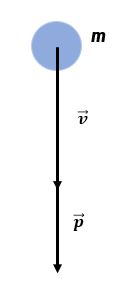
\includegraphics[scale=0.6]{../figs/VN10-PH-29-L-021-1-1.JPG}
		\end{center}
		
		\begin{itemize}
			\item Vecto vận tốc của vật trong chuyển động rơi tự do sau 2 giây có độ lớn 
			\begin{equation*}
				v=g  t =\SI{10}{\meter/\second^2}\cdot\SI{2}{\second}= 20 \ \text{m/s}.
			\end{equation*}
			và có chiều hướng thẳng xuống dưới.
			
			\item Động lượng của vật sau 2 giây là vector có độ lớn 			
			\begin{equation*}
				p=mv= \SI{0.5}{\kilogram}\cdot\SI{20}{\meter/\second}=10\ \text{kg} \cdot \text{m/s}.
			\end{equation*}
			và có chiều từ trên xuống dưới như hình vẽ.
		\end{itemize}
		
		\textbf{Đáp án: C}.
		
		\begin{center}
			\textbf{Câu hỏi tương tự}
		\end{center}
		
		Tại thời điểm $t_0=0$, một vật $m = 1\ \text{kg}$ rơi tự do không vận tốc đầu từ độ cao 80 m xuống đất với $g=10 \text{m/s}^2$. Xác định động lượng của vật tại thời điểm $t = 1\ \text{s}$.
		
		\textbf{Đáp án:} $p=10\ \text{kg} \cdot \text{m/s}$.
	}
\end{dang}

\begin{dang}{Xác định vận tốc hoặc khối lượng của vật dựa vào động lượng}
	\viduii{2}{Một vật có khối lượng $\SI{2}{\kilogram}$ và có động lượng $\SI{6}{kg.m/s}$. Vật đang chuyển động với vận tốc bao nhiêu?
	}
	{	\begin{center}
			\textbf{Hướng dẫn giải}
		\end{center}
		
		Vận tốc của vật: $$p=mv\quad\Rightarrow\quad v=\dfrac{p}{m}=\dfrac{\SI{6}{kg.m/s}}{\SI{2}{\kilogram}}=\SI{3}{m/s}.$$
		
		\begin{center}
			\textbf{Câu hỏi tương tự}
		\end{center}
		
		Một vật có khối lượng $\SI{3}{\kilogram}$ và có động lượng $\SI{6}{kg.m/s}$. Vật đang chuyển động với vận tốc bao nhiêu?
		
		\textbf{Đáp án:} $v=\SI{2}{m/s}$.
	}
	\viduii{2}{Một vật có động lượng $\SI{6}{kg.m/s}$ thì khối lượng của vật là bao nhiêu? Biết vật đang chuyển động với vận tốc $\SI{1}{m/s}$.
	}
	{	\begin{center}
			\textbf{Hướng dẫn giải}
		\end{center}
		
		Khối lượng của vật: $$p=mv\quad\Rightarrow\quad m=\dfrac{p}{v}=\dfrac{\SI{6}{kg.m/s}}{\SI{1}{m/s}}=\SI{6}{kg}.$$
		
		\begin{center}
			\textbf{Câu hỏi tương tự}
		\end{center}
		
		Một vật có động lượng $\SI{60}{kg.m/s}$ thì khối lượng của vật là bao nhiêu? Biết vật đang chuyển động với vận tốc $\SI{36}{km/h}$.
		
		\textbf{Đáp án:} $m=\SI{6}{kg}$.
	}
\end{dang}
\begin{dang}{Xác định tổng động lượng của hệ vật chuyển động cùng phương}
	\viduii{2}{Hệ gồm hai vật có khối lượng lần lượt là $m_1=\SI{3}{kg}$, $m_2=\SI{6}{kg}$, chuyển động với vận tốc có độ lớn lần lượt là $v_1=\SI{2}{m/s}$, $v_2=\SI{1}{m/s}$. Tính độ lớn tổng động lượng của hệ trong trường hợp hai vật chuyển động cùng phương ngược chiều.
	}
	{	\begin{center}
			\textbf{Hướng dẫn giải}
		\end{center}
		
		Động lượng của hệ: $\vec p = \vec p_1 + \vec p_2$.
		
		Vì hai vật chuyển động cùng phương ngược chiều nên $p=|p_1-p_2| = |m_1v_1 - m_2v_2| = 0$.
		
		\begin{center}
			\textbf{Câu hỏi tương tự}
		\end{center}
		
		Hệ gồm hai vật có khối lượng lần lượt là $m_1=\SI{3}{kg}$, $m_2=\SI{6}{kg}$, chuyển động với vận tốc có độ lớn lần lượt là $v_1=\SI{2}{m/s}$, $v_2=\SI{1}{m/s}$. Tính độ lớn tổng động lượng của hệ trong trường hợp hai vật chuyển động cùng phương cùng chiều.
		
		\textbf{Đáp án:} $p=\SI{12}{kg\cdot m/s}$.
	}
	\viduii{2}{Hai vật 1 và 2 chuyển động thẳng đều trên cùng một đường thẳng AB, cùng chiều từ A đến B có khối lượng tốc độ tương ứng với mỗi vật là 5 kg, 36 km/h và 4 kg, 15 m/s. Vectơ tổng động lượng của hệ hai xe có
		\begin{mcq}
			\item độ lớn $240\ \text{kg} \cdot \text{m/s}$; phương là đường thẳng AB chiều từ A đến B.
			\item độ lớn $110\ \text{kg} \cdot \text{m/s}$; phương là đường thẳng AB chiều từ A đến B. 
			\item độ lớn $240\ \text{kg} \cdot \text{m/s}$; phương là đường thẳng AB chiều từ B đến A.
			\item độ lớn $110\ \text{kg} \cdot \text{m/s}$; phương là đường thẳng AB chiều từ B đến A.
		\end{mcq}
	}
	{	\begin{center}
			\textbf{Hướng dẫn giải}
		\end{center}
		
		\begin{center}
			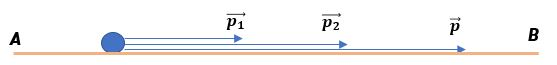
\includegraphics[scale=0.6]{../figs/VN10-PH-29-L-021-2-5.JPG}
		\end{center}
		\begin{itemize}
			\item Vật 1 có động lượng $\vec{p}_1$ có độ lớn 
			\begin{equation*}
				p_1=m_1v_1 =50 \ \text{kg} \cdot \text{m/s}. 
			\end{equation*} 
			và chiều từ A đến B.
			\item Vật 2 có động lượng $\vec{p}_2$ có độ lớn 
			\begin{equation*}
				p_2=m_2v_2 =60 \ \text{kg} \cdot \text{m/s}. 
			\end{equation*}
			và chiều từ A đến B.
			\item Động lượng của hệ là $\vec{p}=\vec{p}_1+\vec{p}_2$ có độ lớn 
			\begin{equation*}
				p=p_1+p_2 =110\ \text{kg} \cdot \text{m/s}. 
			\end{equation*}
			và chiều từ A đến B.
		\end{itemize}
		
		\textbf{Đáp án: B}.
		
		\begin{center}
			\textbf{Câu hỏi tương tự}
		\end{center}
		
		Hai vật 1 và 2 chuyển động thẳng đều trên cùng một đường thẳng AB, vật 1 chuyển động theo chiều từ A đến B với khối lượng 5 kg, tốc độ 54 km/h, vật 2 chuyển động theo chiều từ B đến A với khối lượng 4 kg, tốc độ 36 km/h. Vectơ tổng động lượng của hệ hai vật có
		\begin{mcq}
			\item độ lớn $115\ \text{kg} \cdot \text{m/s}$; phương là đường thẳng AB chiều từ A đến B.
			\item độ lớn $115\ \text{kg} \cdot \text{m/s}$; phương là đường thẳng AB chiều từ B đến A. 
			\item độ lớn $35\ \text{kg} \cdot \text{m/s}$; phương là đường thẳng AB chiều từ B đến A.
			\item độ lớn $35\ \text{kg} \cdot \text{m/s}$; phương là đường thẳng AB chiều từ A đến B.
		\end{mcq}
		
		\textbf{Đáp án: D}.
	}
\end{dang}

\begin{dang}{Xác định tổng động lượng của hệ vật chuyển động khác phương}
	\viduii{2}{Hai vật 1 và 2 chuyển động thẳng đều vận tốc của hai vật tạo với nhau một góc $\beta = 60^\circ$, khối lượng tốc độ tương ứng với mỗi vật là 1 kg, 2 m/s và 3 kg, 4 m/s. Động lượng của hệ hai vật có độ lớn xấp xỉ bằng
		\begin{mcq}(4)
			\item $14\ \text{kg} \cdot \text{m/s}$.	
			\item $11\ \text{kg} \cdot \text{m/s}$.
			\item $13\ \text{kg} \cdot \text{m/s}$.	
			\item $10\ \text{kg} \cdot \text{m/s}$.
		\end{mcq}
	}
	{	\begin{center}
			\textbf{Hướng dẫn giải}
		\end{center}
		
		\begin{center}
			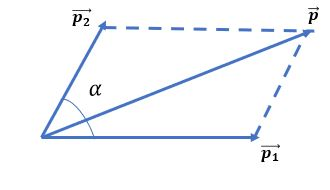
\includegraphics[scale=0.6]{../figs/VN10-PH-29-L-021-2-9.JPG}
		\end{center}
		\begin{itemize}
			\item Độ lớn động lượng của vật 1
			\begin{equation*}
				p_1=m_1v_1 =2\ \text{kg} \cdot \text{m/s}. 
			\end{equation*}
			\item Độ lớn động lượng của vật 1
			\begin{equation*}
				p_2=m_2v_2 =12\ \text{kg} \cdot \text{m/s}. 
			\end{equation*}
			\item Động lượng của hệ hai vật 
			\begin{equation*}
				\vec{p}=\vec{p_1}+\vec{p_2}.
			\end{equation*}
			Do vector động lượng của 2 vật tạo với nhau một góc $\alpha = 60^\circ$ nên độ lớn động lượng của hệ tính bởi 
			\begin{equation*}
				p= \sqrt{p_1^2+p_2^2 +2p_1p_2\cos \alpha}\approx 13\ \text{kg} \cdot \text{m/s}.
			\end{equation*}
		\end{itemize}
		\textbf{Đáp án: C.}
		
		\begin{center}
			\textbf{Câu hỏi tương tự}
		\end{center}
		
		Hai vật 1 và 2 chuyển động thẳng đều vận tốc của hai vật tạo với nhau một góc $\beta = 50^\circ$, khối lượng tốc độ tương ứng với mỗi vật là 1 kg, 4 m/s và 2 kg, 3 m/s. Động lượng của hệ hai vật có độ lớn xấp xỉ bằng
		\begin{mcq}(4)
			\item $9\ \text{kg} \cdot \text{m/s}$.	
			\item $11\ \text{kg} \cdot \text{m/s}$.
			\item $13\ \text{kg} \cdot \text{m/s}$.	
			\item $15\ \text{kg} \cdot \text{m/s}$.
		\end{mcq}
		
		\textbf{Đáp án: A.}
	}
	\viduii{3}{
		Ba vật 1; 2 và 3 chuyển động thẳng đều có khối lượng tốc độ tương ứng với mỗi vật là 1 kg, 2 m/s; 2 kg, 1,5 m/s và 5 kg, $\sqrt {3}$ m/s. Hai vật 1 và 2 chuyển động theo chiều dương trên trục O$x$, vật 3 chuyển động theo chiều dương trên trục O$y$, hệ trục O$xy$ vuông góc. Vectơ tổng động lượng của hệ ba vật có
		\begin{mcq}
			\item độ lớn $14\ \text{kg} \cdot \text{m/s}$; phương tạo với trục O$x$ một góc $\beta = 60^\circ$.
			\item độ lớn $14\ \text{kg} \cdot \text{m/s}$; phương tạo với trục O$x$ một góc $\beta = 30^\circ$. 
			\item độ lớn $10\ \text{kg} \cdot \text{m/s}$; phương tạo với trục O$x$ một góc $\beta = 60^\circ$.
			\item độ lớn $10\ \text{kg} \cdot \text{m/s}$; phương tạo với trục O$x$ một góc $\beta = 30^\circ$.
		\end{mcq}
	}
	{\begin{center}
			\textbf{Hướng dẫn giải}
		\end{center}
		
		\begin{itemize}
			\item Động lượng của vật 1 
			
			+ Độ lớn
			\begin{equation*}
				p_1=m_1v_1=2\ \text{kg} \cdot \text{m/s}. 
			\end{equation*}
			+ Phương trùng với trục Ox, chiều theo chiều dương trục O$x$.
			\item Động lượng của vật 2
			
			+ Độ lớn
			\begin{equation*}
				p_2=m_2v_2=3 \ \text{kg} \cdot \text{m/s}. 
			\end{equation*}
			+ Phương trùng với trục O$x$, chiều theo chiều dương trục O$x$.
			\item Động lượng của vật 3
			
			+ Độ lớn
			\begin{equation*}
				p_3=m_3v_3 =5\sqrt 3 \ \text{kg} \cdot \text{m/s}. 
			\end{equation*}
			+ Phương trùng với trục O$y$, chiều theo chiều dương trục O$y$.
			\item Động lượng của hệ là tổng động lượng của 3 vật 
			\begin{equation*}
				\vec{p} =\vec{p_1}+\vec{p_2} + \vec{p_3}.
			\end{equation*}
			\item Do động lượng của vật 1 và vật 2 cùng phương cùng chiều nên ta nhóm
			\begin{equation*}
				\vec{p} =\vec{p_1}+\vec{p_2} + \vec{p_3} = (\vec{p_1}+\vec{p_2})+ \vec{p_3} = (\vec{p_{12}}+\vec{p_3}).
			\end{equation*}
			\item Động lượng tổng hợp $p_{12}$
			
			+ Độ lớn
			\begin{equation*}
				p_{12} = p_1 +p_2  =5\ \text{kg} \cdot \text{m/s}. 
			\end{equation*}
			+ Phương trùng với trục O$x$, chiều theo chiều dương trục O$x$. 
			\item Động lượng của ba vật 
			
			+ Độ lớn 
			\begin{equation*}
				p = \sqrt {p_{12}^2+p_3^2} =10\ \text{kg} \cdot \text{m/s}. 
			\end{equation*}
			+ Phương là đường chéo của hình chữ nhật tạo với O$x$ góc $\beta$ tính bởi
			\begin{equation*}
				\tan \beta =\dfrac{p_3}{p_{12}} =\sqrt 3 \Rightarrow \beta = 60^\circ. 
			\end{equation*}
			
		\end{itemize}
		
		\textbf{Đáp án: C.}
		
		\begin{center}
			\textbf{Câu hỏi tương tự}
		\end{center}
		
		Ba vật 1; 2 và 3 chuyển động thẳng đều có khối lượng tốc độ tương ứng với mỗi vật là 1 kg, 2 m/s; 2 kg, 1,5 m/s và 5 kg, $\sqrt {3}$ m/s. Vật 1 chuyển động ngược chiều dương trên trục O$x$, vật 2 chuyển động theo chiều dương trên trục O$x$, vật 3 chuyển động theo chiều dương trên trục O$y$, hệ trục O$xy$ vuông góc. Vectơ tổng động lượng của hệ ba vật có
		\begin{mcq}
			\item độ lớn $2\sqrt{3}\ \text{kg} \cdot \text{m/s}$; phương tạo với trục O$x$ một góc $\beta = 6,6^\circ$.
			\item độ lớn $2\sqrt{3}\ \text{kg} \cdot \text{m/s}$; phương tạo với trục O$x$ một góc $\beta = 83,4^\circ$. 
			\item độ lớn $2\sqrt{19}\ \text{kg} \cdot \text{m/s}$; phương tạo với trục O$x$ một góc $\beta = 6,6^\circ$.
			\item độ lớn $2\sqrt{19}\ \text{kg} \cdot \text{m/s}$; phương tạo với trục O$x$ một góc $\beta = 83,4^\circ$.
		\end{mcq}
		
		\textbf{Đáp án: D}.
	}
\end{dang}
\begin{dang}{Xác định độ biến thiên động lượng}
	\viduii{2}{Một quả bóng khối lượng $\SI{500}{g}$, chuyển động theo phương ngang với tốc độ $\SI{10}{m/s}$. Sau khi đập vuông góc vào một bức tường, quả bóng bật trở lại theo phương tới với tốc độ như cũ. Tính độ lớn của độ biến thiên động lượng của quả bóng.
	}
	{	\begin{center}
			\textbf{Hướng dẫn giải}
		\end{center}
		Chọn chiều dương là chiều chuyển động ban đầu của quả bóng. 
		
		Lúc đầu bóng có vận tốc $v_1=\SI{10}{\meter/\second}$ nên có động lượng lúc đầu của bóng 
		\begin{align*}
			p_1=mv_1=\SI{0.5}{\kilogram}\cdot\SI{10}{\meter/\second}=\SI{5}{\kilogram\meter/\second}.
		\end{align*} 
		Sau khi va chạm với tường, bóng chuyển động ngược chiều dương nên có vận tốc $v_2=\SI{-10}{\meter/\second}$ tương ứng với động lượng 
		\begin{align*}
			p_1=mv_2=\SI{0.5}{\kilogram}\cdot\SI{-10}{\meter/\second}=\SI{-5}{\kilogram\meter/\second}.
		\end{align*}
		Độ lớn của độ biến thiên động lượng của quả bóng:
		\begin{align*}
			\Delta p=p_2-p_1=\SI{-5}{\kilogram\meter/\second}-\SI{5}{\kilogram\meter/\second}=\SI{-10}{\kilogram\meter/\second}.
		\end{align*}
		Vậy độ lớn của độ biên thiên động lượng của bóng là \SI{10}{\kilogram \meter/\second}.
		
		
		\begin{center}
			\textbf{Câu hỏi tương tự}
		\end{center}
		
		Một quả bóng khối lượng $\SI{1}{kg}$, chuyển động theo phương ngang với tốc độ $\SI{36}{km/s}$. Sau khi đập vuông góc vào một bức tường, quả bóng bật trở lại theo phương tới với tốc độ như cũ. Tính độ lớn của độ biến thiên động lượng của quả bóng.
		
		\textbf{Đáp án:} $|\Delta p|=\SI{20}{kg\cdot m/s}$.
	}
	\viduii{2}{Một vật khối lượng 1 kg rơi tự do với gia tốc $\text{9,8}\ \text{m/s}^2$ từ trên cao xuống trong khoảng thời gian 0,5 s. Chọn chiều dương hướng thẳng đứng từ trên xuống. Khi đó, xung lượng của lực tác dụng lên vật và độ biến thiên động lượng của vật trong khoảng thời gian nói trên có độ lớn bằng
		\begin{mcq}(2)
			\item $50\ \text{N} \text{s}; 5\ \text{kg} \cdot \text{m/s}$.
			\item $\text{4,9}\ \text{N} \text{s}; \text{4,9}\ \text{kg} \cdot \text{m/s}$.
			\item $10\ \text{N} \text{s}; 10\ \text{kg} \cdot \text{m/s}$.
			\item $\text{0,5}\ \text{N} \text{s}; \text{0,5}\ \text{kg} \cdot \text{m/s}$.
		\end{mcq}
	}
	{	\begin{center}
			\textbf{Hướng dẫn giải}
		\end{center}
		
		\begin{itemize}
			\item Độ lớn xung lượng của lực
			\begin{equation*}
				F \Delta t = mg \Delta t = \text{4,9}\ \text{N}\cdot \text{s}.
			\end{equation*}
			\item Độ lớn độ biến thiên động lượng 
			\begin{equation*}
				\Delta p =F \Delta t = \text{4,9}\ \text{N}\cdot \text{s}=\text{4,9}\ \text{kg} \cdot \text{m/s}.
			\end{equation*}
		\end{itemize}
		
		\textbf{Đáp án: B.}
		
		\begin{center}
			\textbf{Câu hỏi tương tự}
		\end{center}
		
		Một vật khối lượng 1 kg rơi tự do với gia tốc $\text{10}\ \text{m/s}^2$ từ trên cao xuống trong khoảng thời gian 5 s. Chọn chiều dương hướng thẳng đứng từ trên xuống. Khi đó, xung lượng của lực tác dụng lên vật và độ biến thiên động lượng của vật trong khoảng thời gian nói trên có độ lớn bằng
		\begin{mcq}(2)
			\item $50\ \text{N} \text{s}; 50\ \text{kg} \cdot \text{m/s}$.
			\item $\text{5}\ \text{N} \text{s}; \text{5}\ \text{kg} \cdot \text{m/s}$.
			\item $10\ \text{N} \text{s}; 10\ \text{kg} \cdot \text{m/s}$.
			\item $\text{0,5}\ \text{N} \text{s}; \text{0,5}\ \text{kg} \cdot \text{m/s}$.
		\end{mcq}
		
		\textbf{Đáp án: A}.
	}
\end{dang}

\begin{dang}{Xác định độ biến thiên vận tốc, lực, khoảng thời gian mà lực tác dụng}
	\viduii{2}{Một chiếc xe khối lượng 10 kg đang đỗ trên mặt sàn phẳng nhẵn nằm ngang. Tác dụng lên xe một lực đẩy 80 N theo phương ngang để xe chuyển động về phía trước trong khoảng thời gian 2 s, thì độ biến thiên vận tốc của xe trong khoảng thời gian này có độ lớn bằng
		\begin{mcq}(4)
			\item 1,6 m/s.
			\item 0,16 m/s.
			\item 16 m/s.
			\item 160 m/s.
		\end{mcq}
	}
	{	\begin{center}
			\textbf{Hướng dẫn giải}
		\end{center}
		
		Chọn chiều dương là chiều chuyển động của xe lúc đầu.
		
		Dạng khác của định luật II Newton:
		\begin{equation*}
			\vec{F}\Delta t= \Delta \vec{p} =m \Delta \vec{v} \quad\Rightarrow\quad \Delta \vec{v} = \dfrac{\vec{F} \Delta t}{m}.
		\end{equation*}
		Suy ra độ lớn của độ biến thiên vận tốc 
		\begin{equation*}
			\Delta  v=\dfrac{F\Delta t}{m}=\dfrac{\SI{80}{\newton}\cdot\SI{2}{\second}}{\SI{10}{\kilogram}}= 16\ \text{m/s}.
		\end{equation*}
		
		\textbf{Đáp án: C.}
		
		\begin{center}
			\textbf{Câu hỏi tương tự}
		\end{center}
		
		Một vật có trọng lượng 10 N đang đứng yên mặt sàn phẳng nhẵn nằm ngang. Tác dụng lên vật một lực đẩy 80 N theo phương ngang để vật chuyển động về phía trước trong khoảng thời gian 2 s, thì độ biến thiên vận tốc của vật trong khoảng thời gian này có độ lớn bằng
		\begin{mcq}(4)
			\item 1,6 m/s.
			\item 0,16 m/s.
			\item 16 m/s.
			\item 160 m/s.
		\end{mcq}
		
		\textbf{Đáp án: D.}
	}
	\viduii{3}{
		Một quả bóng $\SI{2.5}{\kilogram}$ đập vào tường với vận tốc $\SI{8.5}{\meter/\second}$ và bị bật ngược trở lại với vận tốc $\SI{7.5}{m/s}$. Biết thời gian va chạm là $\SI{0.25}{\second}$. Tìm lực mà tường tác dụng lên quả bóng.
	}
	{\begin{center}
			\textbf{Hướng dẫn giải}
		\end{center}
		Chọn chiều dương là chiều chuyển động lúc đầu của quả bóng. 
		
		Độ biến thiên động lương của quả bóng:
		$$\Delta p =p_2-p_1=mv_2-mv_1=\SI{2.5}{\kilogram}\cdot(\SI{-8.5}{\meter/\second})-\SI{2.5}{\kilogram}\cdot\SI{8.5}{\meter/\second}= \SI{-40}{kg.m/s}.$$
		
		Lưc mà tường tác dụng lên quả bóng: $$F=\dfrac{\Delta p}{\Delta t} =\dfrac{\SI{-40}{\kilogram\meter/\second}}{\SI{0.25}{\second}}= \SI{-160}{N}.$$
		
		\begin{center}
			\textbf{Câu hỏi tương tự}
		\end{center}
		
		Một quả bóng $\SI{2}{\kilogram}$ đập vào tường với vận tốc $\SI{5}{\meter/\second}$ và bị bật ngược trở lại với vận tốc $\SI{4}{m/s}$. Biết thời gian va chạm là $\SI{0.1}{\second}$. Tìm lực mà tường tác dụng lên quả bóng.
		
		\textbf{Đáp án:} $F=\SI{-180}{N}$.
	}
\end{dang}
\section{Trắc nghiệm}
\begin{enumerate}[label=\bfseries Câu \arabic*:]
		\item \mkstar{2}
	
	
	{
		Phát biểu nào sau đây \textbf{sai}?
		\begin{mcq}
			\item Động lượng là một đại lượng vectơ.
			\item Xung lượng của lực là một đại lượng vectơ.
			\item Động lượng tỉ lệ với khối lượng của vật.
			\item Động lượng của vật trong chuyển động tròn đều không đổi.
		\end{mcq}
	}
	
	\hideall
	{	
		\textbf{Đáp án: D.}
		
		Vectơ vận tốc trong chuyển động tròn đều thay đổi theo thời gian nên động lượng của vật trong chuyển động tròn đều thay đổi theo thời gian.
	}
	\item \mkstar{2}
	
	
	{
		Động lượng là đại lượng vectơ
		\begin{mcq}
			\item cùng phương, cùng chiều với vectơ vận tốc. 
			\item cùng phương, ngược chiều với vectơ vận tốc.
			\item có phương vuông góc với vectơ vận tốc.
			\item có phương hợp với vectơ vận tốc một góc $\alpha$ bất kì.
		\end{mcq}
	}
	
	\hideall
	{	
		\textbf{Đáp án: A.}
		
		Động lượng là đại lượng vectơ cùng phương, cùng chiều với vectơ vận tốc.
	}

	\item \mkstar{2}
	
	
	{
		Một quả bóng golf có khối lượng $\SI{46}{g}$ đang nằm yên, sau một cú đánh quả bóng bay lên với tốc độ $\SI{70}{m/s}$. Tính độ lớn trung bình của lực tác dụng vào quả bóng. Biết thời gian tác dụng là $\text{0,5} \cdot 10^{-3}\ \text s.$
		\begin{mcq}(4)
			\item $\SI{6400}{N}$.
			\item $\SI{600}{N}$.
			\item $\SI{400}{N}$.
			\item $\SI{3400}{N}$.
		\end{mcq}
	}
	
	\hideall
	{	\textbf{Đáp án: A.}
		
		Xung lượng của lực
		
		$$\Delta \vec p = \vec {p'} - \vec p \Rightarrow \Delta P = \SI{3,22}{kgm/s}.$$
		
		Lực tác dụng vào quả bóng
		
		$$F = \dfrac{\Delta p}{\Delta t} = \SI{6400}{N}.$$
	}
	\item \mkstar{2}
	
	
	{
		Một electron chuyển động với tốc độ $\xsi{2\cdot 10^7}{m/s}$. Biết khối lượng electron bằng $\text{9,1} \cdot 10^{-31}\ \text{kg}.$ Động lượng của electron bằng
		
		\begin{mcq}(2)
			\item $\text{1,82}\xsi{\cdot 10^{-23}}{kg.m/s}$.
			\item $\text{82}\xsi{\cdot 10^{-23}}{kg.m/s}$.
			\item $\text{1,2}\xsi{\cdot 10^{-23}}{kg.m/s}$.
			\item $\text{1,8}\xsi{\cdot 10^{-23}}{kg.m/s}$.
		\end{mcq}
		
	}
	
	\hideall
	{	
		\textbf{Đáp án: A.}
		
		Động lượng của electron
		
		$$ p  = mv = \text{1,82}\xsi{\cdot 10^{-23}}{kg.m/s}.$$
	}
	\item \mkstar{2}
	
	
	{
		Một quả bóng nặng $\SI{1}{kg}$ đang đứng yên thì cầu thủ chạy đến sút quả bóng thật mạnh. Quả bóng bay đi với vận tốc $\SI{25}{m/s}$. Tính động lượng quả bóng.
		\begin{mcq}(4)
			\item $\SI{15}{kg.m/s}$
			\item $\SI{2}{kg.m/s}$
			\item $\SI{5}{kg.m/s}$
			\item $\SI{25}{kg.m/s}$
		\end{mcq}
	}
	
	\hideall
	{	
		\textbf{Đáp án: D.}
		
		Động lượng của quả bóng: $p=mv=\SI{25}{kg.m/s}$.
	}
\end{enumerate}
\section{Tự luận}
\begin{enumerate}[label=\bfseries Câu \arabic*:]
	
	\item \mkstar{2}
	
	
	{
		Một vật có khối lượng $m=\SI{1}{\kilogram}$ đang chuyển động với vận tốc $v=\SI{2}{\meter/\second}$. Tính động lượng của vật.
	}
	
	\hideall
	{	
		Động lượng của vật: $$p=mv=\SI{2}{kg.m/s}.$$
	}
	\item \mkstar{2}
	
	
	{
		Một vật có khối lượng $\SI{2}{\kilogram}$ và có động lượng $\SI{6}{kg.m/s}$. Vật đang chuyển động với vận tốc bao nhiêu?
	}
	
	\hideall
	{	
		Vận tốc của vật: $$v=\dfrac{p}{m}=\SI{3}{m/s}.$$
	}
	\item \mkstar{2}
	
	
	{
		Một quả bóng có khối lượng $m=\SI{300}{\gram}$ va chạm vào tường và nảy trở lại với cùng tốc độ. Vận tốc bóng trước va chạm là $\SI{5}{\meter/\second}$. Tìm độ biến thiên động lượng.
	}
	
	\hideall
	{	
			Độ biến thiên động lượng của quả bóng:
		$$\Delta \vec p  = \vec p' - \vec p.$$
		
		Vì $\vec p'$ và $\vec p$ cùng phương, ngược chiều nên $$\Delta p = -2p = \SI{-3}{kg.m/s}.$$
	}
	\item \mkstar{2}
	
	
	{
		Một vật có khối lượng $\SI{1}{\kilogram}$ rơi tự do xuống đất trong khoảng thời gian $\SI{0,5}{\second}$. Độ biến thiên động lượng của vật trong khoảng thời gian đó là bao nhiêu? Lấy $g=\SI{10}{\meter/\second^2}$.
	}
	
	\hideall
	{	
		Độ biến thiên vận tốc của vật:
		$$\Delta v = gt = \SI{4.9}{m/s}.$$
		
		Độ biến thiên động lượng của vật: $$\Delta p = m\Delta v = \SI{4.9}{kg.m/s}.$$
	}
	\item \mkstar{2}
	
	
	{
		Một quả bóng $\SI{2.5}{\kilogram}$ đập vào tường với vận tốc $\SI{8.5}{\meter/\second}$ và bị bật ngược trở lại với vận tốc $\SI{7.5}{m/s}$. Biết thời gian va chạm là $\SI{0.25}{\second}$. Tìm lực mà tường tác dụng lên quả bóng.
	}
	
	\hideall
	{	
		Độ biến thiên động lượng của quả bóng:
		$\Delta p = \SI{-40}{kg.m/s}$.
		
		Lưc mà tường tác dụng lên quả bóng: $$F=\dfrac{\Delta p}{\Delta t} = \SI{-160}{N}.$$
	}
	\item \mkstar{2}
	
	
	{
		Một toa xe khối lượng 10 tấn đang chuyển động trên đường ray nằm ngang với vận tốc không đổi $v=\SI{54}{\kilo\meter/\hour}$, người ta tác dụng lên toa xe một lực hãm theo phương ngang. Tính độ lớn trung bình của lực hãm nếu toa xe dừng lại sau
		\begin{enumerate}[label=\alph*)]
			\item 1 phút 40 giây.
			\item 10 giây.
		\end{enumerate}
	}
	
	\hideall
	{	
		\begin{enumerate}[label=\alph*)]
			\item $F=\dfrac{\Delta p}{\Delta t}=\SI{1500}{\newton}$.
			\item $F=\dfrac{\Delta p}{\Delta t}=\SI{15000}{\newton}$.
		\end{enumerate}
	}
	\item \mkstar{2}
	
	
	{
		Một viên đạn khối lượng $\SI{10}{\gram}$ đang bay với vận tốc $\SI{600}{\meter/\second}$ thì gặp một bức tường. Đạn xuyên qua tường trong thời gian $\dfrac{1}{100}\,\text{s}$. Sau khi xuyên qua tường, vận tốc của đạn còn $\SI{200}{\meter/\second}$. Tính lực cản của tường tác dụng lên viên đạn.
	}
	
	\hideall
	{	
		Độ biến thiên động lượng của viên đạn:
		$$\Delta p = m\Delta v = \SI{4}{kg.m/s}.$$
		
		Lực cản của tường tác dụng lên viên đạn: $$F=\dfrac{\Delta p}{\Delta t} = \SI{400}{N}.$$
	}
	\item \mkstar{2}
	
	
	{
		Xác định độ biến thiên động lượng của một vật có khối lượng $\SI{4}{\kilogram}$ sau khoảng thời gian 6 giây. Biết rằng vật chuyển động trên đường thẳng và có phương trình chuyển động là $x=t^2-6t+3$.
	}
	
	\hideall
	{	
		Gia tốc của vật: $a=\SI{2}{m/s^2}$.
		
		Vận tốc ban đầu của vật: $v_0 = \SI{-6}{m/s}$.
		
		Độ biến thiên vận tốc của vật:
		$$\Delta v = v-v_0 = v_0+at-v_0=at = \SI{12}{m/s}.$$
		
		Độ biến thiên động lượng của vật: 
		
		$$\Delta p = m\Delta v = \SI{48}{kg.m/s}.$$
	}
	
		\item \mkstar{2}
	
	
	{
		Một ô tô có khối lượng $\SI{1000}{kg}$, chạy với vận tốc $\SI{54}{km/h}$. Tính động lượng của ô tô.
	}
	
	\hideall
	{	
		Động lượng của ô tô:
		$$p = mv = \SI{15000}{kg.m/s}.$$
	}
	\item \mkstar{2}
	
	
	{
		Một quả bóng khối lượng $\SI{500}{g}$, chuyển động theo phương ngang với tốc độ $\SI{10}{m/s}$. Tính động lượng của quả bóng.
	}
	
	\hideall
	{	
		Động lượng của quả bóng: $$p=mv =\SI{5}{kg.m/s}.$$
	}

\end{enumerate}